% Dokumentace projektu GAL 2014
% Vendula Poncová, xponco00
% Alena Chernikava, xcerni07

\documentclass[a4paper, 11pt, titlepage, final]{article}[3. prosinec 2011]

\newcommand{\uv}[1]{\quotedblbase #1\textquotedblleft}
\newcommand{\mensi}{$<$}
\newcommand{\vetsi}{$>$}

\usepackage[left=1.5cm,text={18cm, 25cm},top=2cm]{geometry}
\usepackage[czech]{babel}
\usepackage[utf8]{inputenc}
\usepackage[IL2]{fontenc}
\usepackage[dvipdf]{graphicx}
\usepackage{color}

\newcommand{\url}[1]{\textit{#1}}
\begin{document}

%%%%%%%%%%%%%%%%%%%%%%%%%%%%%%%%%%%%%%%%%%%%%%%%%%%%%%%%%%%%%%%%%%%%%%%%%
% titulni strana - DON'T TOUCH! MAGIC!

\begin{titlepage}
\begin{center}

\textsc{
\LARGE Fakulta informačních technologií 
\medskip\\
Vysoké učení technické v~Brně}

\vspace{\stretch{0.190}}

{\parbox{5cm}{\centering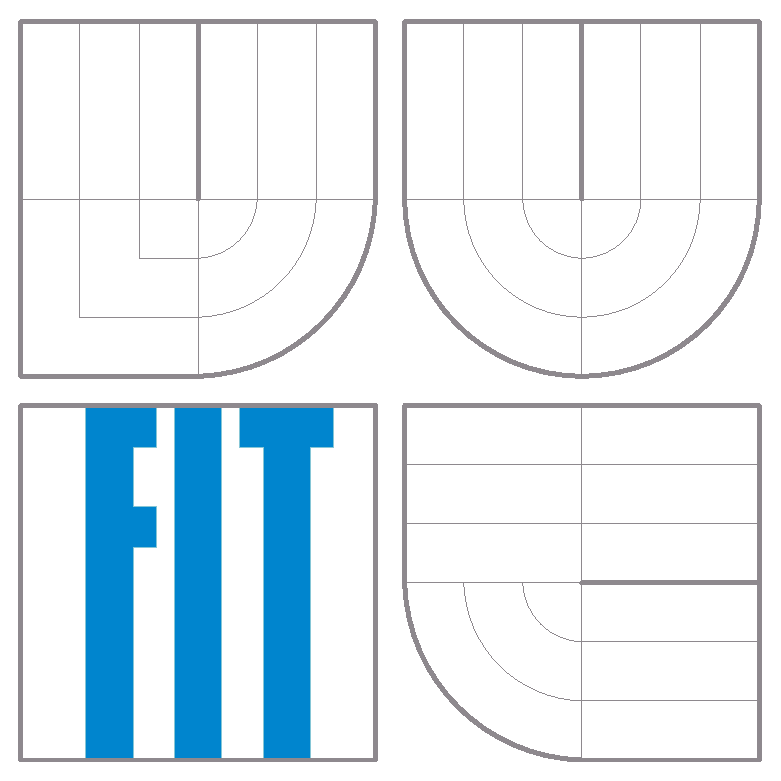
\includegraphics[height=5cm]{img/logo.eps}}}

\vspace{\stretch{0.190}}

{\huge Paralelizace Egerváryho algoritmu} \medskip \\
{\Large Dokumentace projektu do předmětu GAL} 

\vspace{\stretch{0.618}}

\end{center}

{\Large
Tým 33

Vendula Poncová (\texttt{xponco00})

Alena Chernikava (\texttt{xcerni07})
} \hfill {\Large\today}

\end{titlepage}

%%%%%%%%%%%%%%%%%%%%%%%%%%%%%%%%%%%%%%%%%%%%%%%%%%%%%%%%%%%%%%%%%%%%%%%%%
% text dokumentace

\pagestyle{plain}
\pagenumbering{arabic}
\setcounter{page}{1}

%------------------------------------------------------------------------
\section{Úvod}
 
%------------------------------------------------------------------------
\section{Egerváryho algoritmus}

%------------------------------------------------------------------------
\subsection{Sekvenční verze}

\subsubsection*{Návrh}

\subsubsection*{Implementace}

%------------------------------------------------------------------------
\subsection{Paralelní verze}

\subsubsection*{Návrh}

Během návrhu paralelní verze algoritmu jsme vycházely ze sekvenční podoby. Při hledaní M-alternating path se vytváří strom, který je podgrafem vstupního grafu. Po nalezení cesty, případně APS-tree, se pak provádí změny v grafu právě v rámci vytvořeného stromu. Na jiné uzly změny nemají žádný vliv. Graf by proto mohl být zpracováván více procesy, tak, že by procesy vytvářely navzájem disjuktní stromy. Otázkou pak zůstává, jak zajistit, aby stromy byly disjuktní. V ideálním případě, uzel, o který má proces zájem, do žádného stromu nepatří. Proces pak může tento uzel připojit ke svému stromu. Pokud uzel již patří do stromu jiného procesu, dochází ke konfliktu. V Egerváryho algoritmu může dojít ke čtyřem typům takových konfliktů: R-R, R-B, B-B, B-R. Konflikt typu R-B znamená, že proces chce z uzlu typu RED přejít na uzel jiného stromu typu BLUE. 

Typy konfliktů jsou znázorněné na obrázku (OBRÁZEK). Z obrázku jsou zřejmé následující tvrzení: pokud došlo ke konfliktu typu R-R nebo B-B, pak jsme našli M-alternating path z kořenu jednoho stromu do kořenu druhého stromu. Pokud došlo ke konfliktu typu R-B, pak podstrom z uzlu R, je součástí druhého stromu. Pokud došlo ke konfliktu typu R-B, pak z uzlu B vychází více hran, které patří do M, což znamená, že M není matching. Pokud algoritmus pracuje správně, tak by k takovému konfliktu nikdy nemělo dojít. 

Ve dvou případech se tedy výpočet pravděpodobně urychlí. V jednom případě bude třeba jeden strom zahodit a jeho část přiřadit druhému stromu. Pokud ale uvážíme nejhorší možný případ, pak může docházet k tomu, že než se proces dopracuje k nějakému výsledku, bude jiným procesem donucen svůj strom zahodit. Procesy tak budou neustále zahazovat svoje stromy a výpočet se nikdy nezastaví. Je tedy třeba stanovit, kdy má proces právo na uzel stromu jiného procesu. Rozhodujícím parametrem může být například velikost vytvořeného stromu. Pokud proces žádá o uzel stromu s větším počtem uzlů, pak tento proces bude donucen svůj strom zahodit. V opačném případě si přivlastní nárokovaný uzel a druhý proces bude nucen svůj strom zahodit. Pokud stromy budou mít stejný počet uzlů, pak rozhoduje délka života procesu. Potom bude vždy existovat strom s největším počtem uzlů, který má nárok na jakýkoliv uzel, tudíž pro tento strom se výpočet dokončí.


\subsubsection*{Implementace}

%------------------------------------------------------------------------
\section{Experimenty}

%------------------------------------------------------------------------
\section{Závěr}

%------------------------------------------------------------------------
\end{document}

% end of file
